%=======================================================================
% riscv-trace.tex
%-----------------------------------------------------------------------

\documentclass[twoside,11pt]{book}
\usepackage{footnote}

\makesavenoteenv{tabulary}
\setcounter{tocdepth}{4}
\setcounter{secnumdepth}{4}

% Fix copy/pasting of ligatures in Acrobat
\input{glyphtounicode.tex}
\pdfgentounicode=1 %

% Package includes

\usepackage[T1]{fontenc}
\usepackage{graphicx}
\usepackage{geometry}
\usepackage{array}
\usepackage{colortbl}
\usepackage[colorlinks=true,linkcolor=blue]{hyperref}
\usepackage{placeins}
\usepackage{bbding}
\usepackage{longtable}
\usepackage{multirow}
\usepackage{float}
\usepackage{pdfpages}
\usepackage{placeins}
\usepackage{tabulary}
%\usepackage{listings}
\usepackage{algorithmicx}
\usepackage{program}
\usepackage[nochapter]{vhistory}
%\usepackage{tablefootnote}

% If LaTeX just doesn't do what I want, buy http://www.amazon.com/gp/product/0201362996

% Used for tables that can span pages:
\usepackage{xtab}

% Keep spacing normal in enumerated instead of adding extra space between
% items.
\usepackage{enumitem}
%\setlist{nolistsep}

\newenvironment{steps}[1]
  {
     \vspace{1ex}
     \noindent
     #1
     \begin{enumerate}
  }
  {
     \end{enumerate}
     \vspace{1ex}
 }

% Setup margins

\setlength{\topmargin}{-0.5in}
\setlength{\textheight}{9in}
\setlength{\oddsidemargin}{0in}
\setlength{\evensidemargin}{0in}
\setlength{\textwidth}{6.5in}

% Useful macros

\newcommand{\note}[1]{{\bf [ NOTE: #1 ]}}
\newcommand{\fixme}[1]{{\bf [ FIXME: #1 ]}}
\newcommand{\todo}[1]{\marginpar{\footnotesize #1}}

\newcommand{\wunits}[2]{\mbox{#1\,#2}}
\newcommand{\um}{\mbox{$\mu$m}}
\newcommand{\xum}[1]{\wunits{#1}{\um}}
\newcommand{\by}[2]{\mbox{#1$\times$#2}}
\newcommand{\byby}[3]{\mbox{#1$\times$#2$\times$#3}}

\newlength\savedwidth
\newcommand\whline[1]{%
  \noalign{%
    \global\savedwidth\arrayrulewidth\global\arrayrulewidth 1.5pt%
  }%
  \cline{#1}%
  \noalign{\vskip\arrayrulewidth}%
  \noalign{\global\arrayrulewidth\savedwidth}%
}

% Custom list environments

\newenvironment{tightlist}
{\begin{itemize}
 \setlength{\parsep}{0pt}
 \setlength{\itemsep}{-2pt}}
{\end{itemize}}

\newenvironment{titledtightlist}[1]
{\noindent
 ~~\textbf{#1}
 \begin{itemize}
 \setlength{\parsep}{0pt}
 \setlength{\itemsep}{-2pt}}
{\end{itemize}}

\newenvironment{commentary}
{ \vspace{-0.2in}
  \begin{quotation}
  \noindent
  \small \em
  \rule{\linewidth}{1pt}\\
}
{ 
  \end{quotation}
  \vspace{-0.2in}
}

% Other commands and parameters

\pagestyle{myheadings}
\setlength{\parindent}{0in}
\setlength{\parskip}{10pt}
\sloppy

% Commands for register format figures.

% New column types to use in tabular environment for instruction formats.
% Allocate 0.18in per bit.
\newcolumntype{I}{>{\centering\arraybackslash}p{0.18in}}
% Two-bit centered column.
\newcolumntype{W}{>{\centering\arraybackslash}p{0.36in}}
% Three-bit centered column.
\newcolumntype{F}{>{\centering\arraybackslash}p{0.54in}}
% Four-bit centered column.
\newcolumntype{Y}{>{\centering\arraybackslash}p{0.72in}}
% Five-bit centered column.
\newcolumntype{R}{>{\centering\arraybackslash}p{0.9in}}
% Six-bit centered column.
\newcolumntype{S}{>{\centering\arraybackslash}p{1.08in}}
% Seven-bit centered column.
\newcolumntype{O}{>{\centering\arraybackslash}p{1.26in}}
% Eight-bit centered column.
\newcolumntype{E}{>{\centering\arraybackslash}p{1.44in}}
% Ten-bit centered column.
\newcolumntype{T}{>{\centering\arraybackslash}p{1.8in}}
% Twelve-bit centered column.
\newcolumntype{M}{>{\centering\arraybackslash}p{2.2in}}
% Sixteen-bit centered column.
\newcolumntype{K}{>{\centering\arraybackslash}p{2.88in}}
% Twenty-bit centered column.
\newcolumntype{U}{>{\centering\arraybackslash}p{3.6in}}
% Twenty-bit centered column.
\newcolumntype{L}{>{\centering\arraybackslash}p{3.6in}}
% Twenty-five-bit centered column.
\newcolumntype{J}{>{\centering\arraybackslash}p{4.5in}}

\newcommand{\instbit}[1]{\mbox{\scriptsize #1}}
\newcommand{\instbitrange}[2]{~\instbit{#1} \hfill \instbit{#2}~}
\newcommand{\reglabel}[1]{\hfill {\tt #1}\hfill\ }

\newcommand{\wiri}{\textbf{WIRI}}
\newcommand{\wpri}{\textbf{WPRI}}
\newcommand{\wlrl}{\textbf{WLRL}}
\newcommand{\warl}{\textbf{WARL}}





% All registers are named here. That way when we rename one we'll get errors if
% there are still references to the old name.

\usepackage{makeidx}
\makeindex

\usepackage{xspace}
\usepackage{placeins}

\newcommand{\versionnum}{0.026-DRAFT}

%%% This file is generated by Makefile.
%%% Do not edit this file!\n%%%
    \gdef\GITHash{c0e7304d2c91f410c97d62fce7c0e0b4639e9343}    \gdef\GITAbrHash{c0e7304}    \gdef\GITAuthorDate{Sat Nov 23 12:31:13 2019 +0000}    \gdef\GITAuthorName{Iain Robertson}

\begin{document}
\setcounter{footnote}{0}

\title{RISC-V Processor Trace\\
Version \versionnum\\
\GITHash
}

\author{
  Gajinder Panesar, Iain Robertson \\
 \textless gajinder.panesar@ultrasoc.com\textgreater, \textless iain.robertson@ultrasoc.com\textgreater
 \and
 UltraSoC Technologies Ltd.
}


\maketitle

\markboth{RISC-V Processor Trace Version \versionnum}
{RISC-V Processor Trace Version \versionnum}
\thispagestyle{empty}

\frontmatter

\tableofcontents
\listoffigures
\listoftables

\mainmatter

\chapter{Introduction}
\label{sec:intro}

In complex systems understanding program behavior is not easy.
Unsurprisingly in such systems, software sometimes does not behave as
expected. This may be due to a number of factors, for example,
interactions with other cores, software, peripherals, realtime
events, poor implementations or some combination of all of the above.

It is not always possible to use a debugger to observe behavior of a
running system as this is intrusive.  Providing visibility of program
execution is important.  This needs to be done without swamping the
system with vast amounts of data.

One method of achieving this is via a Processor Branch Trace.

This works by tracking execution from a known start address and sending
messages about the address deltas taken by the program. These deltas are
typically introduced by jump, call, return and branch type instructions,
although interrupts and exceptions are also types of deltas.

Conceptually, the system has one or more of the following fundamental components:

\begin{itemize}
  \item
    A core with an instruction trace interface that outputs all relevant
    information to allow the successful creation of a processor branch trace and more.
    This is a high bandwidth interface: in most implementations, it will supply
    a large amount of data (instruction address, instruction type, context information, ...)
    for each core execution clock cycle;
  \item
    A hardware encoder that connects to this instruction trace interface and compresses
    the information into lower bandwidth trace packets;
  \item
    A transmission channel to transmit or a memory to store these trace packets;
  \item
    A decoder, usually software on an external PC, that takes in the trace
    packets and, with knowledge of the program binary that's running on the
    originating hart, reconstructs the program flow. This decoding step can
    be done off-line or in real-time while the hart is executing.
\end{itemize}

In RISC-V, all instructions are executed unconditionally or at least
their execution can be determined based on the program binary. The
instructions between the deltas can all be assumed to be executed
sequentially. Because of this, there is no need to report sequential 
instructions in the trace, only whether the branches were taken or not
and the address of taken indirect branches or jumps. If the program
counter is changed by an amount that cannot be determined from the
execution binary, the trace decoder needs to be given the destination
address (i.e. the address of the next valid instruction).  Examples of
this are indirect branches or jumps, where the next instruction
address is determined by the contents of a register rather than a
constant embedded in the program binary.

Interrupts generally occur asynchronously to the program's execution
rather than intentionally as a result of a specific instruction or
event.  Exceptions can be thought of in the same way, even though they
can be typically linked back to a specific instruction address.  The
decoder generally does not know where an interrupt occurs in the
instruction sequence, so the trace encoder must report the address
where normal program flow ceased, as well as give an indication of the
asynchronous destination which may be as simple as reporting the
exception type.  When an interrupt or exception occurs, or the
processor is halted, the final instruction retired beforehand must be
included in the trace.

This document serves to specify the ingress port (the signals between
the RISC-V core and the encoder), compressed branch trace algorithm and
the packet format used to encapsulate the compressed branch trace
information.

\section{Terminology} \label{sec:terminology}

The following terms have a specific meaning in this specification.

\begin{itemize}
  \item \textbf{ATB}: Arm trace bus
  \item \textbf{branch}: an instruction which conditionally changes the execution flow
  \item \textbf{CSR}: control/status register
  \item \textbf{decoder}: a piece of software that takes the trace packets emitted by the encoder and 
    reconstructs the execution flow of the code executed by the RISC-V hart
  \item \textbf{delta}: a change in the program counter that is other than the difference between two instructions placed consecutively in memory
  \item \textbf{discontinuity}: another name for 'delta' (see above)
  \item \textbf{ELF}: executable and linkable format
  \item \textbf{encoder}: a piece of hardware that takes in instruction execution information from a RISC-V hart and transforms it into trace packets
  \item \textbf{exception}: an unusual condition occurring at run time associated with an instruction in a RISC-V hart
  \item \textbf{hart}: a RISC-V hardware thread
  \item \textbf{interrupt}: an external asynchronous event that may cause a RISC-V hart to experience an unexpected transfer of control
  \item \textbf{ISA}: instruction set architecture
  \item \textbf{jump}: an instruction which unconditionally changes the execution flow
  \item \textbf{direct jump}: an instruction which unconditionally changes the execution flow by changing the PC by a constant value
  \item \textbf{indirect jump}: an instruction which unconditionally changes the execution flow by changing the PC to a computed value
  \item \textbf{inferable jump}: a jump where the target address is supplied via a constant embedded within the jump opcode
  \item \textbf{uninferable jump}: a jump which is not inferable (see above)
  \item \textbf{LSB}: least significant bit
  \item \textbf{MSB}: most significant bit
  \item \textbf{packet}: the atomic unit of encoded trace information emitted by the encoder
  \item \textbf{PC}: program counter
  \item \textbf{program counter}: a register containing the address of the instruction being executed
  \item \textbf{retire}: the final stage of executing an instruction, when the machine state is updated (sometimes referred to as 'commit' or 'graduate')
  \item \textbf{trap}: the transfer of control to a trap handler caused by either an exception or an interrupt
  \item \textbf{updiscon}: contraction of 'uninferable PC discontinuity'
\end{itemize}

\section{Nomenclature}

In the following sections items in \textbf{bold} are signals or
fields within a packet.

Items in \textbf{\textit{bold italics}} are mnemonics for instructions or CSRs defined in the RISC-V ISA

Items in \textit{italics} with names ending \textit{'\_p'} refer to parameters either built into the
hardware or configurable hardware values.



\chapter{Branch Trace} \label{Branch Trace}


Instruction delta tracing, also known as branch tracing, works by
tracking execution from a known start address by sending information
about the deltas taken by the program. Deltas are typically introduced
by jump, call, return and branch type instructions, although
interrupts and exceptions are also types of deltas.

Instruction delta tracing provides an efficient encoding of an
instruction sequence by exploiting the deterministic way the processor
behaves based on the program it is executing.

The approach relies on
an offline copy of the program binary being available to the decoder, so it
is generally unsuitable for either dynamic (self-modifying) programs
or those where access to the program binary is prohibited.

While the program binary is sufficient, access to the assembly or
higher-level source code will improve the ability of the decoder to present
the decoded trace in the debugger by annotating the traced instructions with
source code line numbers and labels, variable names etc.

This approach can be extended to cope with small sections of
deterministically dynamic code by arranging for the decoder to request
instruction memory from the target. Memory lookups generally lead to a
prohibitive reduction in performance, although they are suitable for
examining modest jump tables, such as the exception/interrupt vector
pointers of an operating system which may be adjusted at boot up and
when services are registered.  Both static and dynamically linked
programs can be traced using this approach. Statically linked programs
are straightforward as they generally operate in a known address
space, often mapping directly to physical memory. Dynamically linked
programs require the debugger to keep track of memory allocation
operations using either trace or stop-mode debugging.

\section{Instruction delta trace concepts} \label{Trace Concepts}

\subsection{Sequential instructions} \label{Sequential Instructions}

For instruction set architectures such as RISC-V where all instructions are executed
unconditionally or at least their execution can be determined based on
the program binary, the instructions between the deltas are assumed to be
executed sequentially. Consequently, there is no need
to report them in the trace. The trace only needs to contain whether
branches were taken or not, the addresses of taken indirect jumps, or
other program counter discontinuities.

\subsection{Uninferable PC discontinuities} \label{uninfpc}

An uninferable program counter discontinuity is a program counter change
that can not be inferred from the program binary alone. For these cases,
the instruction delta trace must include a destination address: the
address of the next valid instruction.

Indirect jumps are an example of this, where
the next instruction address is determined by the contents of a
register rather than a constant embedded in the program binary.  In this 
case, the address of the instruction following the jump (also known as the
jump target) must be traced.

Interrupts and exceptions are another form of uninferable PC discontinuity;
these are discussed in detail below.

\subsection{Branches} \label{branches}

A branch is an instruction where a jump is conditional on the
value of a register or a flag. For a decoder to able to follow program flow,
the trace must include whether a branch was taken or not.

For a direct branch, where the destination address is encoded in the 
program binary (either as a constant, or as a constant offset from the
program counter), no further information is required.
Direct branches are the only type of branch that is supported by the
RISC-V ISA.

\subsection{Interrupts and exceptions} \label{interruptsexceptions}

Interrupts are a different type of delta that generally occur
asynchronously to the program's execution rather than intentionally as
a result of a specific instruction or event. Exceptions can be thought
of in the same way, even though they can be typically linked back to a
specific instruction address.

The decoder generally does not know
where an interrupt occured in the instruction sequence, so the trace
must report the address where normal program flow ceased, as well as
give an indication of the asynchronous destination which may be as
simple as reporting the exception type.  When an interrupt or
exception occurs, the final instruction retired beforehand must be traced.  
Following this the next valid instruction address (the first of the
trap handler) must be traced.

Note: not all exceptions and interrupts cause traps (see 
section~\ref{sec:terminology} for definitions). Most notably, 
floating point exceptions and disabled interrupts do not trap.
If an exception or interrupt doesn't trap, the program counter does not
change. So, there is no need to trace all exceptions/interrupts, just
traps.  In this document, interrupts and exceptions are only traced when 
they cause traps to be taken.

\subsection{Synchronization} \label{synchronization}

In order to make the trace robust there must be regular
synchronization points within the trace. Synchronization is accomplished by
sending a full valued instruction address (and potentially a context
identifier). The decoder and debugger may also benefit from sending
the reason for synchronizing. The frequency of synchronization is a
trade-off between robustness and trace bandwidth.

The instruction trace encoder needs to synchronise fully:

\begin{itemize}

\item For the first instruction traced after reset or resume from halt;
\item Any time that an instruction is traced and the previous instruction was not traced;
\item If the instruction is the first of an interrupt service routine or
exception handler.
\item After a prolonged period of time.
\end{itemize}

\subsection{End of trace} \label{sec:endoftrace}

If tracing stops for any reason, the address of the final traced instruction must be output.

Some examples of why tracing may stop are: 
\begin{itemize}
  \item The hart may be halted (entered debug mode);
  \item The hart may be reset;
  \item Encoding may be stopped (for example via a \textit{Trace-off} trigger - see section~\ref{sec:trigger});
  \item The matching criteria for any filtering capabilities implemented by the encoder may no longer be met;
  \item The encoder may be disabled.
\end{itemize}

\section{Optional and run-time configurable modes} \label{optional}

An instruction trace encoder may support multiple tracing modes.
To ensure that the decoder treats the incoming packets
correctly, it needs to be informed of the current active configuration.
The configuration is reported by a packet that is issued by the encoder
whenever the encoder configuration is changed.

Here are common examples of such modes:

\begin{itemize}
  \item delta address mode:
    program counter discontinuities are encoded as differences instead of absolute address values.
  \item full address mode:
    program counter discontinuities are encoded as absolute address values.
  \item implicit exception mode:
    the destination address of an exception (i.e. the address of the exception trap) is assumed to 
    be known by the decoder, and thus not encoded in the trace.
  \item Sequentially inferable jump mode:
    The target of an indirect jump can be inferred by considering the combined effect of two instructions. 
  \item implicit return mode:
    the destination address of function call returns is derived from a call stack, and thus not encoded
    in the trace.
  \item branch prediction mode:
    branches that are predicted correctly by an encoder branch predictor (and an identical copy in the decoder)
    are not encoded as taken/non-taken, but as a more efficient branch count number.
  \item Jump target cache mode:
    Rather than reporting the address of an uninferable jump target, efficiency can be improved by caching
    recent jump targets, and reporting the cache entry index instead.
\end{itemize}

Modes may have associated parameters; see Table~\ref{tab:parameters} for further details.

All modes are optional apart from delta address mode, which must be supported.

\subsection{Delta address mode} \label{sec:delta-address}

Related parameters: None

In delta address mode, addresses are encoded as the difference between the actual address of 
the current instruction and the actual address of the instruction reported in the 
previous packet that contained an address.  This differential encoding requires fewer bits than 
the full address, and thus results in more efficient trace compression.

\subsection{Full address mode} \label{sec:full-address}

Related parameters: None

In full address mode, all addresses in the trace are encoded as absolute addresses instead
of in differential form. This kind of encoding is always less efficient, but it can be a useful 
debugging aid for software decoder developers.

\subsection{Implicit exception mode} \label{sec:implicit-exception}

Related parameters: None

The RISC-V Privileged ISA specification stores exception handler base
addresses in the \textbf{\textit{utvec/stvec/mtvec}} CSR registers.
In some RISC-V implementations, the lower address bits are stored in
the \textbf{\textit{ucause/scause/mcause}} CSR registers.

By default, both the \textbf{\textit{*tvec}} and \textbf{\textit{*cause}} 
values are reported when an exception or interrupt occurs.

The implicit exception mode omits \textbf{\textit{*tvec}} (the trap handler address), 
from the trace and thus improves efficiency.

This mode can only be used if the decoder can infer the address of the trap handler
from just the exception cause.

\subsection{Sequentially inferable jump mode} \label{sec:si-jump}

Related parameters: \textit{sijump\_p}.

By default, the target of an indirect jump is always considered an uninferable PC discontinuity.  
However, if the register that specifies the jump target was loaded with a constant then it
can be considered inferable under some circumstances.  The hart must identify jumps with 
sequentially inferable targets and provide this information separately to the encoder.  The
final decision as to whether to treat the jump as inferable or not must be made by the encoder.
Both the constant load and the jump must be traced in order for the decoder to be able to
infer the jump target.  See Section~\ref{Jump Classes} for details of what constitutes a sequentially
inferable jump.

\subsection{Implicit return mode} \label{sec:implicit-return}

Related parameters: \textit{call\_counter\_size\_p}, \textit{return\_stack\_size\_p}, \textit{itype\_width\_p}.

Although a function return is usually an indirect jump, well behaved programs return to the
point in the program from which the function was called using a standard calling convention.
For those programs, it is possible to determine the execution path without being explicitly notified
of the destination address of the return.  The implicit return mode can result in very
significant improvements in trace encoder efficiency.

Returns can only be treated as inferable if the associated call has already been reported in
an earlier packet.  The encoder must ensure that this is the case.  This can be accomplished
by utilizing a counter to keep track of the number of nested calls being traced.  The counter
increments on calls (but not tail calls), and decrements on returns (see Section~\ref{Jump Classes}
for definitions).  The counter will not over or underflow, and is reset to 0 whenever a
synchronization packet is sent.  Returns will be treated as inferable and will not generate a trace
packet if the count is non-zero (i.e. the associated call was already reported in an earlier packet).

Such a scheme is low cost, and will work as long as programs are "well behaved".  The encoder does not check that the
return address is actually that of the instruction following the associated call.  As such, any program that
modifies return addresses cannot be traced using this mode with this minimal implementation.

Alternatively, the encoder can maintain a stack of expected return addresses, and only treat a
return as inferable if the actual return address matches the prediction.  This is fully robust for all
programs, but is more expensive to implement.  In this case, if a return address does not match the prediction, 
it must be reported explicitly via a packet, along with the number of return addresses
currently on the stack.  This ensures that the decoder can determine which return is being reported. 

\subsection{Branch prediction mode} \label{sec:branch-prediction}

Related parameters: \textit{bpred\_size\_p}.

Without branch prediction, the outcome of each executed branch is stored in
a branch map: a bit vector in which the taken/non-taken status of each branch is stored in
chronological order.

While this encoding is efficient, at 1 bit per branch, there are some cases where this
can still result in a relatively large volume of trace packets.  For example:

\begin{itemize}
  \item Executing tight loops of code containing no uninferable jumps.  Each iteration of the loop will add a bit 
  to the branch map;
  \item Sitting in an idle loop waiting for an interrupt.  This produces large amounts of trace when nothing of 
  any interest is actually happening!  
  \item Breakpoints, which in some implementations also spin in an idle loop.
\end{itemize}

A significant coding efficiency can be obtained by the addition of a branch predictor in the encoder. To keep
the encoder and decoder synchronized, a predictor with identical behavior will need to be implemented in the decoder
software.

The predictor shall comprise a lookup table of 2\textsuperscript{\textit{bpred\_size\_p}} entries.  
Each entry is indexed by bits \textit{bpred\_size\_p}:1 of the instruction address (or \textit{bpred\_size\_p}+1:2 if 
compressed instructions aren't supported), 
and each contains a 2-bit prediction state:
\begin{itemize}
  \item 00: predict not taken, transition to 01 if prediction fails;
  \item 01: predict not taken, transition to 00 if prediction succeeds, else 11;
  \item 11: predict taken, transition to 10 if prediction fails;
  \item 10: predict taken, transition to 11 if prediction succeeds, else 00.
\end{itemize}

The MSB represents the predicted outcome, the LSB the most recent actual outcome.  The prediction must fail twice
for the predicted value to change.

The lookup table entries are initialized to 01 when a synchronization packet is sent.

Other predictors, such as the gShare predictor (see Hennessy \& Patterson), should be considered.  Some further
experimentation is needed to determine the benefits of different lookup table sizes and predictor algorithms.


\subsection{Jump target cache mode} \label{sec:jump-cache}

Related parameters: \textit{cache\_size\_p}.

By default, the target address of an uninferable jump is output in the trace, usually in differential
form.  If the same function is called repeatedly, (for example, in a loop), the same address will be output 
repeatedly.  

An efficiency gain can be obtained by the addition of a jump target cache to the encoder.  To keep
the encoder and decoder synchronized, a cache with identical behavior will need to be implemented in the 
decoder software.  Even a small cache can provide significant improvement.

The cache shall comprise 2\textsuperscript{\textit{cache\_size\_p}} entries, each of which can contain
an instruction address.  It will be direct mapped, with each entry indexed by bits \textit{cache\_size\_p}:1 
of the instruction address (or \textit{cache\_size\_p}+1:2 if compressed instructions aren't supported).   

Each uninferable jump target is first compared with the entry at its index in the cache.  If it is 
found in the cache, the index number is traced rather than the target address.  If it is not found in 
the cache, the entry at that index is replaced with the current instruction address.

The cache entries are all invalidated when a synchronization packet is sent.  



\chapter{Ingress Port} \label{Interface}

\section{Interface requirements}
This section describes in general terms the information which must be passed from the RISC-V hart to the trace encoder,
and distinguishes between what is mandatory, and what is optional.

The following information is mandatory:

\begin{itemize}
  \item The number of instructions that are being retired;
  \item Whether there has been an exception or interrupt, and if so the cause (from the \textbf{\textit{ucause/scause/mcause}} CSR)
        and trap value (from the \textbf{\textit{utval/stval/mtval}} CSR);
  \item The current privilege level of the RISC-V hart;
  \item The \textit{instruction\_type} of retired instructions for:
    \begin{itemize}
      \item Jumps with a target that cannot be inferred from the source code;
      \item Taken branches;
      \item Return from exception or interrupt (\textbf{\textit{*ret}} instructions).
    \end{itemize}
  \item The \textit{instruction\_address} for:
    \begin{itemize}
      \item Jumps with a target that \textit{cannot} be inferred from the source code;
      \item Taken branches;
      \item The instruction executed immediately after a jump or taken branch (also referred to as the target or destination of the jump or taken branch);
      \item The last instruction executed before an exception or interrupt;
      \item Exceptions;
      \item The first instruction executed following an exception or interrupt;
      \item The last instruction executed before a privilege change;
      \item The first instruction executed following a privilege change;
      \item The first and last instruction being retired.
    \end{itemize}
  \item The number of nontaken branches being retired.
\end{itemize}

The following information is optional:

\begin{itemize}
  \item Context information:
    \begin{itemize}
      \item The context and/or hart ID;
      \item The type of action to take when context changes.
    \end{itemize}
  \item The \textit{instruction\_type} of instructions for:
    \begin{itemize}
      \item Calls with a target that \textit{cannot} be inferred from the source code;
      \item Calls with a target that \textit{can} be inferred from the source code;
      \item Tail-calls with a target that \textit{cannot} be inferred from the source code;
      \item Tail-calls with a target that \textit{can} be inferred from the source code;
      \item Returns with a target that \textit{cannot} be inferred from the source code;
      \item Returns with a target that \textit{can} be inferred from the source code;
      \item Co-routine swap;
      \item Jumps which don't fit any of the above classifications with a target that \textit{cannot} be inferred from the source code;
      \item Jumps which don't fit any of the above classifications with a target that \textit{can} be inferred from the source code;
      \item Nontaken branches.
    \end{itemize}
  \item If context is supported then the \textit{instruction\_address} for:
    \begin{itemize}
      \item The last instruction executed before a context change;
      \item The first instruction executed following a context change.
    \end{itemize}
  \item Whether jump targets are sequentially inferable or not.
\end{itemize}

The mandatory information is the bare-minimum required to implement the branch trace algorithm outlined in Chapter~\ref{Algorithm}.  
The optional information facilitates alternative or improved trace algorithms:

\begin{itemize}
  \item Implicit return mode (see Section~\ref{sec:implicit-return}) requires the encoder to keep track of the number of nested 
    function calls, and to do this it must be aware of all calls and returns regardless of whether the target can be inferred or not;
  \item A simpler algorithm useful for basic code profiling would only report function calls and returns, again 
    regardless of whether the target can be inferred or not;
  \item Branch prediction techniques can be used to further improve the encoder efficiency, particularly for loops 
    (see Section~\ref{sec:branch-prediction}).  This requires the encoder to be aware of the address of all branches, whether
    they are taken or not.
  \item Uninferable jumps can be treated as inferable (which don't need to be reported in the trace output) if both the jump 
    and the preceding instruction which loads the target into a register have been traced.
\end{itemize}

\subsection{Jump classification and target inference} \label{Jump Classes}

Jumps are classified as \textit{inferable}, or \textit{uninferable}.  An \textit{inferable} jump has a target which can be
deduced from the binary executable or representation thereof (e.g. ELF).  For the purposes of this specification, the following 
strict definition applies:

If the target of a jump is supplied via a constant embedded within the jump opcode, it is classified as \textit{inferable}.
Jumps which are not \textit{inferable} are by definition \textit{uninferable}.

However, there are some jump targets which can still be deduced from the binary executable by considering pairs of instructions
even though by the above definition they are classified as uninferable.  Specifically, jump targets that are supplied via

\begin{itemize}
  \item an \textbf{\textit{lui}} or \textbf{\textit{c.lui}} (a register which contains a constant), or
  \item an \textbf{\textit{auipc}} (a register which contains a constant offset from the PC).
\end{itemize}

Such jump targets are classified as \textit{sequentially inferable} if the pair of instructions are executed consecutively 
(i.e. the \textbf{\textit{auipc}}, \textbf{\textit{lui}} or \textbf{\textit{c.lui}} immediately precedes the jump).  Note:
the restriction that the instructions are executed consecutively is necessary in order to minimize the additional signalling
needed between the hart and the encoder, and should have a minimal impact on trace efficiency as it is anticipated that
consecutive execution will be the norm. Support for sequentially inferable jumps is optional.

Jumps may optionally be further classified according to the recommended calling convention:

\begin{itemize}
  \item \textit{Calls}: 
    \begin{itemize}
      \item \textbf{\textit{jal}} x1;
      \item \textbf{\textit{jal}} x5;
      \item \textbf{\textit{jalr}} x1, rs  where rs != x1;
      \item \textbf{\textit{jalr}} x5, rs  where rs != x5;
      \item \textbf{\textit{c.jalr}} rs1.
    \end{itemize}
  \item \textit{Tail-calls}: 
    \begin{itemize}
      \item \textbf{\textit{jalr}} x0, rs where rs != x1 and rs != x5;
      \item \textbf{\textit{c.jr}} rs1 where rs1 != x1 and rs1 != x5.
    \end{itemize}
  \item \textit{Returns}: 
    \begin{itemize}
      \item \textbf{\textit{jalr}} x0, rs where rs == x1 or rs == x5;
      \item \textbf{\textit{c.jr}} rs1 where rs1 == x1 or rs1 == x5.
    \end{itemize}
  \item \textit{Co-routine swap}: 
    \begin{itemize}
      \item \textbf{\textit{jalr}} x1, x1;
      \item \textbf{\textit{jalr}} x5, x5.
    \end{itemize}
  \item \textit{Other}: 
    \begin{itemize}
      \item \textbf{\textit{jal}} rd where rd != x1 and rd != x5;
      \item \textbf{\textit{jalr}} rd, rs where rd != x0 and rd != x1 and rd != x5.
    \end{itemize}
\end{itemize}

\section{Instruction interface}
This section describes the interface between a RISC-V hart and the
trace encoder that conveys the information described in the previous section.  
Signals are assigned to one of the  following groups:

\begin{itemize}
  \item M: Mandatory.  The interface must include an instance of this signal.
  \item O: Optional.  The interface may include an instance of this signal.
  \item MR: Mandatory, may be replicated. For harts that can retire a maximum of N taken branches per clock
    cycle, the interface must include N instances of this signal.
  \item OR: Optional, may be replicated. For harts that can retire a maximum of N taken branches per clock
    cycle, the interface must include zero or N instances of this signal.
  \item BR: Block, may be replicated.  Mandatory for harts that can retire multiple instructions in a block.  
    Replication as per OR.  If omitted, the interface must include SR group signals instead.
  \item SR: Single, may be replicated.  Mandatory for harts that can only retire one instruction in a block.  
    Replication as per OR.  If omitted, the interface must include BR group signals instead.
\end{itemize}

\begin{table}[htp]
    \centering
    \caption{Instruction interface signals}
    \label{tab:common-ingress}
    \begin{tabulary}{\textwidth}{|l|l|p{80mm}|}
        \hline
        \textbf{Signal} & \textbf{Group} & \textbf{Function} \\
        \hline
        \textbf{itype}[\textit{itype\_width\_p}-1:0] & MR & Termination type of the instruction block (see Section~\ref{Jump Classes} for definitions of codes 6 - 15):\newline
        0: Final instruction in the block is none of the other named \textbf{itype} codes;\newline
        1: Exception. An exception occurred following the final retired instruction in the block;\newline
        2: Interrupt. An interrupt occurred following the final retired instruction in the block;\newline
        3: Exception return;\newline
        4: Nontaken branch;\newline
        5: Taken branch;\newline
        6: reserved;\newline
        7: Co-routine swap;\newline
        8: Uninferable call;\newline
        9: Inferrable call;\newline
        10: Uninferable tail-call;\newline
        11: Inferrable tail-call;\newline
        12: Uninferable return;\newline
        13: Inferrable return;\newline
        14: Other uninferable jump;\newline
        15: Other inferable jump.\\
        \hline
        \textbf{cause}[\textit{ecause\_width\_p}-1:0] & M & Exception or interrupt cause (\textbf{\textit{ucause/scause/ mcause}}).
        Ignored unless \textbf {itype}=1 or 2.\\
        \hline
        \textbf{tval}[\textit{iaddress\_width\_p}-1:0] & M & The associated trap value, e.g. the
        faulting virtual address for address exceptions, as would be
        written to the \textbf{utval/stval/mtval} CSR. Future optional extensions may define \textbf{tval} 
        to provide ancillary information in cases where it currently supplies zero.
        Ignored unless \textbf{itype}=1 or 2.\\
        \hline
        \textbf{priv}[\textit{privilege\_width\_p}-1:0] & M & Privilege level for all instructions in this block.\\
        \hline
        \textbf{iaddr}[\textit{iaddress\_width\_p}-1:0] & MR & The address of the 1st instruction retired in this block.
        Invalid if \textbf{iretire}=0 \\
        \hline
        \textbf{context}[\textit{context\_width\_p}-1:0] & O & Context for all instructions in this block.\\
        \hline
        \textbf{ctype}[\textit{ctype\_width\_p}-1:0] & O & Reporting behavior for \textbf{context}:\newline
        0: Don't report; \newline
        1: Report imprecisely;\newline
        2: Report precisely;\newline
        3: Report as asynchronous discontinuity.\\
        \hline
        \textbf{ntkn}[\textit{ntkn\_width\_p}-1:0] & OR & Number of nontaken branches in this block.\\
        \hline
        \textbf{sijump} & OR & If \textbf{itype} indicates that this block ends with an uninferable discontinuity, setting this signal to 1 
        indicates that it is sequentially inferable and may be treated as inferable by the encoder if the preceding 
        \textbf{\textit{auipc}}, \textbf{\textit{lui}} or \textbf{\textit{c.lui}} has been traced.  
        Must be zero for \textbf{itype} codes other than 8, 10, 12 or 14.\\
        \hline
    \end{tabulary}
\end{table}

\begin{table}[htp]
    \centering
    \caption{Instruction interface signals - multiple retirement per block}
    \label{tab:multi-ingress}
    \begin{tabulary}{\textwidth}{|l|l|p{80mm}|}
        \hline
        \textbf{Signal} & \textbf{Group} & \textbf{Function} \\
        \hline
        \textbf{iretire}[\textit{iretire\_width\_p}-1:0] & BR & Number of halfwords represented by instructions retired in this block.\\
        \hline
        \textbf{ilastsize}[\textit{ilastsize\_width\_p}-1:0] & BR & The size of the last retired instruction is 2\textsuperscript{\textbf{ilastsize}} half-words.\\
        \hline
    \end{tabulary}
\end{table}

\begin{table}[htp]
    \centering
    \caption{Instruction interface signals - single retirement per block}
    \label{tab:single-ingress}
    \begin{tabulary}{\textwidth}{|l|l|p{110mm}|}
        \hline
        \textbf{Signal} & \textbf{Group} & \textbf{Function} \\
        \hline
        \textbf{iretire}[0:0] & SR & Number of instructions retired in this block (0 or 1).\\
        \hline
    \end{tabulary}
\end{table}

Tables~\ref{tab:common-ingress} and ~\ref{tab:multi-ingress}
list the signals in the interface designed to efficiently support retirement of multiple 
instructions per cycle.  The following discussion describes the multiple-retirement behavior.  
However, for harts that can only retire one instruction at a time, the signalling can be 
simplified, and this is discussed subsequently in Section~\ref{sec:single-retire}.  

The information presented on the ingress port represents a contiguous
block of instructions starting at \textbf{iaddr}, all of which retired
in the same cycle. Note if \textbf{itype} is 1 or 2 (indicating an
exception or an interrupt), the number of instructions retired may be
zero. \textbf{cause} and \textbf{tval} are only defined if
\textbf{itype} is 1 or 2. If \textbf{iretire}=0 and \textbf{itype}=0,
the values of all other signals are undefined.

\textbf{iretire} contains the number of half-words represented by
instructions retired in this block, and \textbf{ilastsize} the size of the last
instruction.  Half-words rather than instruction count enables the encoder to easily compute the address of
the last instruction in the block without having access to the size of every 
instruction in the block.  

If address translation is enabled, \textbf{iaddr} is a virtual
address, else it is a physical address. Virtual addresses narrower
than \textit{iaddress\_width\_p} bits must be sign-extended to make
computation of differential addresses easier, and physical addresses
narrower than \textit{iaddress\_width\_p} bits must be zero-extended.

Harts can retire multiple non-taken branches per clock cycle, indicated via \textbf{ntkn}.
However, a consequence of this is that the encoder will be unaware of the addresses of some non-taken branches, 
which will prevent the use of a branch predictor to improve compression (see Section~\ref{sec:branch-prediction}).
For harts that can only retire a maximum of one non-taken branch per clock cycle,
\textbf{ntkn} can be omitted, provided all non-taken branches are indicated via \textbf{itype}.  
The number of non-taken branches is \textbf{ntkn} if \textbf{ntkn} is non-zero, or 1 if \textbf{itype} = 4 and \textbf{ntkn} is zero.
In other words, if for example \textbf{ntkn} is 2 and \textbf{itype} = 4, the encoder will interpret this as 2 non-taken branches,
not 3.

For harts that can retire a maximum of N taken branches per clock
cycle, the signal groups MR, OR and either BR or SR must be replicated N times. 
Signal group 0 represents information about the oldest instruction block, and group N-1
represents the newest instruction block. The interface supports no more
than one privilege, context, exception or interrupt per cycle and so signals in
groups M and O are not replicated. Furthermore, \textbf{itype} can only
take the value 1 or 2 in one of the signal groups, and this must be
the newest valid group (i.e. \textbf{iretire} and \textbf{itype} must
be zero for higher numbered groups). If fewer than N taken branches
are retired in a cycle, then lower numbered groups must be used
first. For example, if there is one taken branch, use only group 0, if
there are two taken branches, instructions up to the 1st taken branch
must be reported in group 0 and instructions up to the 2nd taken branch
must be reported in group 1 and so on.

\textbf{sijump} is optional and may be omitted if the hart does not implement the logic to detect
sequentially inferable jumps.  If the encoder offers an \textbf{sijump} input it must also provide a
parameter to indicate whether the input is connected to a hart that implements this capability, or
tied off.  This is to ensure the decoder can be made aware of the hart's capability.  Enabling 
sequentially inferable jump mode in the encoder and decoder when the hart does not support it will
prevent correct reconstruction by the decoder. 

The \textbf{context} field can be used to convey any additional information to the decoder.  For example:

\begin{itemize}
  \item The hart ID;
  \item The software thread ID;
  \item It could be used to convey the values of CSRs to the decoder by setting \textbf{context} to the 
    CSR number and value when a CSR is written.
\end{itemize}

Table~\ref{tab:context-type} specifies the actions for the various \textbf{ctype} values.  A typical 
behaviour would be for this signal to remain zero except on the 1st retirement after a context change.

\begin{table}[htp]
    \centering
    \caption{Context type \textbf{ctype} values and corresponding actions}
    \label{tab:context-type}
    \begin{tabulary}{\textwidth}{|l|l|p{90mm}|}
        \hline
        \textbf{Type} & \textbf{Value} & \textbf{Actions} \\
        \hline
        Unreported & 0 & No action (don't report context).\\
        \hline
        Report context imprecisely & 1 & An example would be a SW thread change.\newline
        Report the new context value at the earliest convenient opportunity.\newline
        It is reported without any address information, and the assumption is that the precise 
        point of context change can be deduced from the source code (e.g. a CSR write). \\
        \hline
        Report context precisely  & 2 & Report the address of the 1st instruction retired in this block, and the new context.\newline
        If there were unreported branches beforehand, these need to be reported first.\newline
        Treated the same as a privilege change.\\
        \hline
        Report context as an & 3 &  An example would be a change of hart.\\
        asynchronous discontinuity & & 
        Need to report the last instruction executed on the previous context, as well as the 1st on the new context.\newline
        Treated the same as an exception.\\
        \hline
    \end{tabulary}
\end{table}

\subsection{Simplifications for single-retirement} \label{sec:single-retire}

For harts that can only retire one instruction at a time, the interface can be simplified to
the signals listed in tables~\ref{tab:common-ingress} and ~\ref{tab:single-ingress}.  The 
simplifications can be summarized as follows:
 
\begin{itemize}
  \item As the number of instructions that are retired in a block is only 0 or 1, the 
    encoder does not need information to enable it to deduce the address of the last instruction 
    retired (it is the same as the 1st and only instruction retired).  So 
    \textbf{ilastsize} is not necessary, and \textbf{iretire} simply indicates whether an
    instruction retired or not;
  \item As the number of non-taken branches retired is never more than 1, and can always
    be indicated via \textbf{itype}, \textbf{ntkn} is not necessary.
\end{itemize}

The parameter \textit{retires\_p} which indicates to the encoder the maximum number of 
instructions that can be retired per cycle can be used by an encoder capable of supporting single or 
multiple retirement to select the appropriate interpretation of \textbf{iretire}.  
\textbf{ilastsize} and \textbf{ntkn} encoder inputs must be tied low when attached to a single-retirement
hart that does not provide these outputs.


\subsection{Alternative multiple-retirement interface configurations}

For a hart that can retire multiple instructions per cycle, but no more than one taken branch, the preferred 
solution is to use one instance of signals from groups BR, MR and OR.  However, an alternative approach would 
be to provide explicit details of every instruction retired by using N instances of signals from groups
SR, MR and OR (replicating the single retirement example N times).  

\subsection{Optional sideband signals}

Optional sideband signals may be included to provide additional functionality, as described in
tables \ref{tab:ingress-side-band} and \ref{tab:egress-side-band}.

Note, any user defined information that needs to be output by the encoder
will need to be applied via the \textbf{context} input.

\begin{table}[htp]
    \centering
    \caption{Optional sideband encoder ingress signals}
    \label{tab:ingress-side-band}
    \begin{tabulary}{\textwidth}{|l|l|p{90mm}|}
        \hline
        \textbf{Signal} & \textbf{Group} & \textbf{Function} \\
        \hline
        \textbf{impdef}[\textit{impdef\_width\_p}-1:0] & O &  Implementation defined sideband signals.  A typical use for
        these would be for filtering (see Chapter~\ref{ch:filtering}.\\
        \hline
        \textbf{trigger}[2:0] & OR & A pulse on bit 0 will cause the encoder to start tracing, and continue until further 
        notice, subject to other filtering criteria also being met.\newline
        A pulse on bit 1 will cause the encoder to stop tracing until further notice.  See section~\ref{sec:trigger}).\\
        \hline
        \textbf{halted} & O & Hart is halted.  Upon assertion, the encoder will output a packet to report the address 
        of the last instruction retired before halting, followed by a support packet to indicate that tracing has stopped. 
        Upon deassertion, the encoder will start tracing again, commencing with a synchronization packet.\\
        \hline
        \textbf{reset} & O & Hart is in reset.  Provided the encoder is in a different reset domain to the hart, this
        allows the encoder to indicate that tracing has ended on entry to reset, and restarted on exit.  
        Behavior is as described above for halt.\\
        \hline
    \end{tabulary}
\end{table}

\begin{table}[htp]
    \centering
    \caption{Optional sideband encoder egress signals}
    \label{tab:egress-side-band}
    \begin{tabulary}{\textwidth}{|l|l|p{130mm}|}
        \hline
        \textbf{Signal} & \textbf{Group} & \textbf{Function} \\
        \hline
        \textbf{stall} & O & Stall request to hart.  Some applications may require lossless trace, which can be achieved by
        using this signal to stall the hart if the trace encoder is unable to output a trace packet (for example due to 
        back-pressure from the packet transport infrastructure).\\
        \hline
    \end{tabulary}
\end{table}

\FloatBarrier
\subsection{Using trigger outputs from the Debug Module} \label{sec:trigger}

The debug module of the RISC-V hart may have a trigger unit. This defines a match control register
(\textbf{\textit{mcontrol}}) containing a 4-bit \textbf{action} field, and reserves codes 2 - 5 
of this field for trace use.  
These action codes are hereby defined as shown in table \ref{tab:debugModuleTriggerSupport}.
If implemented, each action must generate a pulse on an output from the hart, on the same cycle as the instruction which
caused the trigger is retired.  

\begin{table}[!h]
    \centering
    \caption{Debug Module trigger support (\textbf{\textit{mcontrol}} \textbf{action})}
    \label{tab:debugModuleTriggerSupport}
    \begin{tabulary}{\textwidth}{|l|p{120mm}|}
        \hline
        \textbf {Value} & \textbf {Description} \\
        \hline
        2 & \textit{Trace-on}.  This should be connected to 
        \textbf{trigger[0]} if the encoder provides it. \\ 
        \hline
        3 & \textit{Trace-off}.  This should be connected to 
        \textbf{trigger[1]} if the encoder provides it. \\
        \hline
        4 & \textit{Trace-notify}.  This should be connected to 
        \textbf{trigger[2]} if the encoder provides it. This will cause the encoder to output
        a packet containing the address of the last instruction in the block if it is enabled.\\
        \hline
    \end{tabulary}
\end{table}

Trace-on and Trace-off actions provide a means for the hart to control when tracing occurs.  
Trace-notify provides  means to ensure that a specified instruction is explicitly reported.  
This capability is sometimes known as a watchpoint.

\subsection{Example retirement sequences}

\begin{table}[htp]
    \centering
    \caption{Example 1 : 9 Instructions retired over three cycles, 2 branches} 
    \label{tab:signal-block-9-instructions-2-branches}
    \begin{tabulary}{\textwidth}{|l|l|}
        \hline
        \textbf {Retired} & \textbf {Instruction Trace Block} \\
        \hline
        1000: \textbf{\textit{divuw}} &  \textbf{iretire}=7, \textbf{iaddr}=0x1000, \textbf{ntkn}=0, \textbf{itype}=8\\
        1004: \textbf{\textit{add}} &  \\
        1008: \textbf{\textit{or}} &  \\
        100C: \textbf{\textit{c.jalr}} &  \\
        \hline
        0940: \textbf{\textit{addi}} &  \textbf{iretire}=4, \textbf{iaddr}=0x0940, \textbf{ntkn}=1, \textbf{itype}=5\\
        0944: \textbf{\textit{c.beq}} &  \\
        0946: \textbf{\textit{c.bnez}} &  \\
        \hline
        0988: \textbf{\textit{lbu}} &  \textbf{iretire}=4, \textbf{iaddr}=0x0988, \textbf{ntkn}=0, \textbf{itype}=0\\
        098C: \textbf{\textit{csrrw}} &  \\
        \hline
    \end{tabulary}
\end{table}


\chapter{Filtering} \label{ch:filtering}

The contents of this chapter are informative only.

Filtering provides a mechanism to control whether the encoder should produce trace.  For example,
it may be desirable to trace:

\begin{itemize}
  \item When the instruction address is within a particular range;
  \item Starting from one instruction address and continuing until a second instruction address;
  \item For one or more specified privilege levels;
  \item For a particular context or range of contexts;
  \item Exception and/or interrupt handlers for specified exception causes or with particular \textbf{tval} values;
  \item Based on values applied to the \textbf{impdef} or \textbf{trigger} signals;
  \item For a fixed period of time
  \item etc.
\end{itemize}

How this is accomplished is implementation specific.  

One suggested implementation provides: 

\begin{itemize}
  \item Comparators offering a range of arithmetic options (<, >, =, !=, etc) for \textbf{iaddress}, 
    \textbf{context} and \textbf{tval} inputs;
  \item Multiple choice selection for \textbf{priv} and \textbf{cause} inputs;
  \item Masked matching for \textbf{interrupt} and \textbf{impdef} inputs;
  \item The ability to enable tracing when \textbf{trigger[0]} is asserted, and continue tracing 
    until \textbf{trigger[0]} is asserted (see Section~\ref{sec:trigger}).
\end{itemize}



\chapter{Example Algorithm} \label{Algorithm}

An example algorithm for compressed branch trace is given in figure~\ref{fig:algo}. 
In the diagram, the following terms are used:

\begin{itemize}
  \item \textit{te\_inst.} The name of the packet type emitted by the encoder (see Chapter~\ref{packets});
  \item \textit{inst.}  Abbreviation for 'instruction';
  \item \textit{updiscon.}  Uninferable PC discontinuity.  This identifies an instruction that
    causes the program counter to be changed by an amount that cannot be predicted from the
    source code alone (\textbf{itype} values 8, 10, 12 or 14);
  \item \textit{Qualified?}  An instruction that meets the filtering criteria is qualified, and will be traced;
  \item \textit{Branch?} Is the instruction a branch or not (\textbf{itype} values 4 or 5, or a non-zero \textbf{ntkn});
  \item \textit{branch map.}  A vector where each bit represents the outcome of a branch.  A 0 indicates the
    branch was taken, a 1 indicates that it was not;
  \item \textit{e\_ccd.} An exception has been signalled, or context has changed and
    should be treated as an uninferable PC discontinuity (see Table~\ref{tab:context-type});
  \item \textit{ppch.} Privilege has changed, or context has changed and needs to be 
    reported precisely (see Table~\ref{tab:context-type});
  \item \textit{ppch\_br.} As above, but branch map not empty;
  \item \textit{er\_ccdn.}  Instruction retirement and exception signalled on the same cycle, 
    or context has changed and should be treated as an uninferable PC discontinuity, or
    context notification (see Table~\ref{tab:context-type});
  \item \textit{exc\_only.}  Exception signalled without simultaneous retirement;
  \item \textit{cci.}  context change that can be reported imprecisely (see Table~\ref{tab:context-type});
  \item \textit{resync count.} A counter used to keep track of when it is necessary to send 
    a synchronization packet (see Section~\ref{sec:resync});
  \item \textit{max\_resync.}  The resync counter value that schedules a synchronization packet (see Section~\ref{sec:resync});
  \item \textit{resync\_br.} The resync counter has reached the maximum value and there are
    entries in the branch map that have not yet been output (see Section~\ref{sec:resync}).
\end{itemize}

\begin{figure}
\begin{center}
  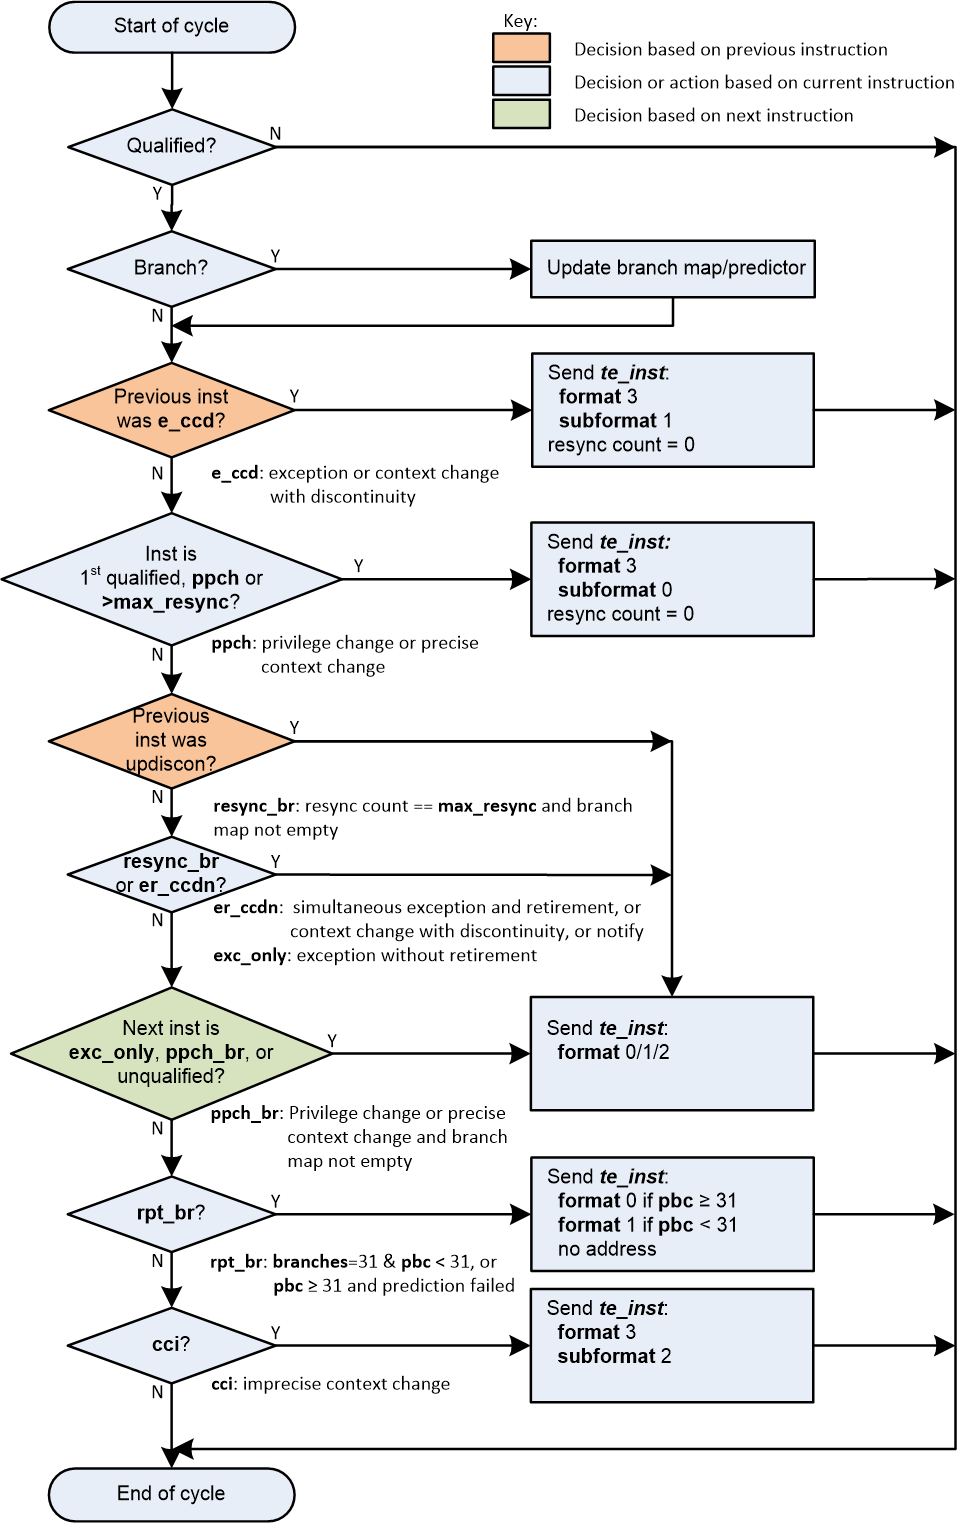
\includegraphics[height=23cm, width=15cm]{algo.png}
  \caption{Delta Mode 1 instruction trace algorithm}
  \label{fig:algo}
\end{center}
\end{figure}

Figure~\ref{fig:algo} shows instruction by instruction behavior, as would be
seen in a single-retirement system only.  Whilst the ingress port allows the RISC-V core to
provide information on multiple retiring instructions simultaneously, the resultant packet
sequence generated by the encoder must be the same as if retiring one instruction at a time.

A 3-stage pipeline is assumed, such that the encoder has 
visibility of the current, previous and next instructions.  All packets are generated using 
information relating to the current instruction.  The orange diamonds indicate decisions 
based on the previous (or last) instruction, the green diamond indicates a decision based on the
next instruction, and all other diamonds are based on the current instruction.

Additionally, the encoder can generate one further packet type, not shown on the diagram for 
clarity.  The \textit{support} packet (format 3, subformat 3 - see Chapter~\ref{packets}) is 
sent when:

\begin{itemize}
  \item The encoder is enabled or disabled, or its configuration is changed, 
    to inform the decoder of the operating mode of the encoder
  \item After the last qualified instruction has been traced, to inform the decoder that 
    tracing has stopped;
  \item If trace packets are lost (for example if the buffer into which packets are being 
    written fills up.  In this situation, the 1st packet 
    loaded into the buffer when space next becomes available should be a \textit{support} 
    packet.  Following this, tracing will resume with a sync packet.
\end{itemize}

Note: if the \textbf{halted} or \textbf{reset} sideband signals are asserted (see Table~\ref{tab:ingress-side-band})
the encoder will behave as if it has received an unqualified instruction (output \textit{te\_inst}
reporting the address of the last instruction, followed by \textit{te\_support});


\section{Full vs Differential Addresses} \label{addresses}
Addresses can be output in one of two ways: \textit{full} or \textit{differential}.

\begin{itemize}
  \item The \textit{full} address is the actual address of the current instruction;
  \item The \textit{differential} address is the difference between the actual address of 
    the current instruction and the actual address of the instruction reported in the 
    previous packet that contained an address.
\end{itemize}

Packet formats 1 and 2 include a differential address, whilst format 3 includes the full address.

If the optional full address mode is enabled (see Section~\ref{sec:full-address}), all packet formats
will include a full address.

\section{Format selection} \label{format-selection}

In all cases but one, the packet format (3) is determined only by a 'yes' outcome from the 
associated decision.  The choice between formats 1 or 2 for the case in the middle of the 
diagram needs further explanation.  

If there are no branches that need to be reported, packet format 2 is used.  

If there are branches to report, format 1 is used.

If branch prediction is supported and is enabled, then there is a choice of whether to output a 
full branch map, or a count of correctly predicted branches.  In order to choose the count, the number 
of correctly predicted branches must be at least 31.  If there are 31 unreported branches (i.e. the branch
map is full), but not all of them were predicted correctly, then the branch map will be output.
If all 31 unreported branches were correctly predicted, then the encoder starts counting
subsequent correct predictions, and will output a count under the following conditions:

\begin{itemize}
  \item A branch is mis-predicted.  The count value will be the number of correctly predicted branches, 
    minus 31.  \textbf{branch\_fmt} will be 01, indicating that the next branch failed its prediction.
   No address information is provided;
  \item An updiscon, interrupt or exception requires the encoder to output an address.  In this case 
    the encoder will output the branch count (number of correctly predicted branches, minus 31) with 
    \textbf{branch\_fmt} set to 10.  The packet also contains \textbf{mispred}, indicating whether 
    prediction of the next branch failed.
  \item The branch count reaches its maximum value (0xffff).  Again, \textbf{branch\_fmt} will be set to 10.
    Strictly speaking an address isn't required for this case, but it will occur so rarely that the bandwidth 
    impact can be ignored
\end{itemize}

Packet formats 1 and 2 are organized so that the address is usually the final field.  Minimizing the 
number of bits required to represent the address reduces the total packet size and significantly
improves efficiency.  See Chapter~\ref{packets}.

\section{Resynchronisation} \label{sec:resync}

Per Section~\ref{synchronization}, a format 3 synchronisation packet must be output after "a prolonged
period of time". The exact mechanism for
determining this is not specified, but options might be to count the number of \textit{te\_inst} packets emitted, 
or the number of clock cycles elapsed, since the last synchronization message was sent.

When the resync is required, the primary objective is to output a format 3 packet, so that the decoder can 
start tracing from that point without needing any of the history.  However, if the decoder is already synced, 
then it is also required that it can continue to follow the execution path up to and through the format 3 packet 
seamlessly.  As such, before outputting a format 3 packet, it is necessary to output a format 1 packet for the 
preceding instruction if there are any unreported branches (because format 3 does not contain a branch map).  
The format 3 will be sent if the resync timer has been exceeded.  On the cycle before this (when the resync timer 
value has been exactly reached), a format 1 will be generated if the branch map is not empty.

\chapter{Trace Encoder Output Packets} \label{packets}

The bulk of this section describes the payload of packets output from the Trace Encoder.  
The infrastructure used to transport these packets is outside the scope of this document, and
as such the manner in which packets are encapsulated for transport is not specified.
However, the following information must be provided to the encapsulator:

\begin{itemize}
  \item The packet type;
  \item The packet length, in bytes;
  \item The packet payload.
\end{itemize}

Two example transport schemes are the UltraSoC Messaging Infrastructure, and the Arm Trace Bus.
Figure~\ref{fig:packet-format} shows the encapsulation used for the UltraSoC infrastructure:
\begin{itemize}
  \item The header byte contains a 5-bit field specifying the payload length in bytes, a 2-bit
    field indicating the "flow" (destination routing indicator), and a bit to indicate whether
    an optional 16-bit timestamp is present;
  \item The index field indicates the source of the packet.  The number of bits is system dependent,
    And the initial value emitted by the trace encoder is zero (it gets adjusted as it propagates 
    through the infrastructure);
  \item An optional 2-byte timestamp;
  \item The packet payload.
\end{itemize}

\begin{figure}[h]
  \begin{center}
    \includegraphics[height=1cm, width=9cm]{newPacket.jpg}
    \caption{Example encapsulated packet format}
    \label{fig:packet-format}
  \end{center}
\end{figure}


Alternatively, for ATB, the source of the packet is indicated by the \textbf{ATID} bus field, and there is
no equivalent of "flow", so an example encapsulation might be:
\begin{itemize}
  \item A 5-bit field specifying the payload length in bytes
  \item A bit to indicate whether an optional 16-bit timestamp is present;
  \item An optional 2-byte timestamp;
  \item The packet payload.
\end{itemize}
It may be desirable for packets to start aligned to an ATB word, in which the \textbf{ATBYTES} bus field
in the last beat of a packet can be used to indicate the number of valid bytes.

The remainder of this section describes the contents of the payload
portion which should be independent of the infrastructure.  In each table, the fields are listed in
transmission order: first field in the table is transmitted first, and multi-bit fields are 
transmitted LSB first.

This packet payload format is used to output encoded instruction
trace.  Three different formats are used according to the needs of the
encoding algorithm. The following tables show the format of the
payload - i.e. excluding any encapsulation.

In order to achieve best performance, actual packet lengths may be adjusted using 'sign based compression'.
At the very minimum this should be applied to the address field of format 1 and 2 packets, but ideally will 
be applied to the whole packet, regardless of format.  This technique eliminates identical bits from the most 
significant end of the packet, and adjusts the length of the packet accordingly.  A decoder receiving this 
shortened packet can reconstruct the original full-length packet by sign-extending from the most significant
received bit.  

Where the payload length given in the following tables, or after applying sign-based compression, is not a 
multiple of whole bytes in length, the payload must be sign-extended to the nearest byte boundary.

Whilst offering maximum encoding efficiency, variable length packets can present some challenges,
specifically in terms of identifying where the boundaries between packets occur either when packed
packets are written to memory, or when packets are streamed offchip via a communications channel.  Two 
potential solutions to this are as follows:

\begin{itemize}
  \item If the maximum packet payload length is 2\textsuperscript{N}-1 (for example, if N is 5, then the maximum length is
    31 bytes), and the minimum packet payload length is 1, then a sequence of at least 2\textsuperscript{N} zero 
    bytes cannot occur within a packet payload, and therefore the first non-zero byte seen after a sequence of 
    at least 2\textsuperscript{N} zero bytes must be the first byte of a packet.  This approach can be used for
    alignment in either memory or a data stream;
  \item An alternative approach suitable for packets written to memory is to divide memory into blocks of M bytes
    (e.g. 1kbyte blocks), and write packets to memory such that the first byte in every block is always the first
    byte of a packet.  This means packets cannot span block boundaries, and so zero bytes must be used to pad between 
    the end of the last message in a block and the block boundary.
\end{itemize}

\section{Format 3 packets} \label{sec:format3}

Format 3 packets are used for synchronization, reporting context and supporting information.  There are 4
sub-formats.

Throughout this document, the term "synchronization packet" is used.  This refers specifically to format 3, 
subformat 0 and subformat 1 packets.

\section{Format 3 subformat 0 - Synchronisation} \label{sec:format30}

This packet contains all the information the decoder needs to fully identify an instruction.  It is sent for
the first traced instruction (unless that instruction also happens to be a the first in an exception handler), 
and when resynchronization has been scheduled by expiry of the resynchronisation timer.

\begin{table}[htp]
  \centering
  \caption{Packet format 3, subformat 0}
  \label{tab:te_inst3}
  \begin{tabulary}{\textwidth}{|l|p{35mm}|p{90mm}|}
    \hline
    {\bf Field name} & {\bf Bits} & {\bf Description} \\
    \hline
    \textbf{format} & 2 & 11 (sync): synchronisation\\
    \hline
    \textbf{subformat} & 2 & 00 (start): Start of tracing, or resync \\
    \hline
    \textbf{branch} & 1 & Set to 0 if the address points to a branch instruction, and the branch was taken.  
              Set to 1 if the instruction is not a branch or if the branch is not taken. \\
    \hline
    \textbf{privilege} & \textit {privilege\_width\_p} & 
                The privilege level of the reported instruction\\
    \hline
    \textbf{context} &  \textit {context\_width\_p}, 
               or 0 if \textit {nocontext\_p} is 1 & 
               The instruction context \\
    \hline
    \textbf{address} & \textit {iaddress\_width\_p - iaddress\_lsb\_p} & 
              Full instruction address.  Address alignment is determined by \textit {iaddress\_lsb\_p} Address must be left shifted in order to recreate original byte address. \\
    \hline
  \end{tabulary}
\end{table}

\subsection{Format 3 \textbf{branch} field}

This bit indicates the taken/not taken status in the case where the reported address points to a branch instruction.
Overall efficiency would be slightly improved if this bit was removed, and the branch status was instead 
"carried over" and reported in the next \textit{te\_inst} packet.  This was considered, but there are several
pathological cases where this approach fails.  Consider for example the situation where the first traced instruction
is a branch, and this is then followed immediately by an exception.  This results in format 3 packets being generated 
on two consecutive instructions.  The second packet does not contain a branch
map, so there is no way to report the branch status of the 1st branch, apart from by inserting a format 1 packet in 
between.  There are two issues with this:

\begin{itemize}
  \item It would require the generation of 2 packets on the same cycle, which adds significant additional complexity
    to the encoder;
  \item It would complicate the algorithm shown in figure~\ref{fig:algo}. 
\end{itemize}

\FloatBarrier
\section{Format 3 subformat 1 - Exception} \label{sec:format31}

This packet also contains all the information the decoder needs to fully identify an instruction.
It is sent following an exception, and as well as reporting the address of the exception handler, it also 
includes the exception cause and the address of the faulted instruction.

If the implicit exception mode is enabled (see section~\ref{sec:implicit-exception}), the address is omited.

\begin{table}[htp]
  \centering
  \caption{Packet format 3, subformat 1}
  \label{tab:te_inst3}
  \begin{tabulary}{\textwidth}{|l|p{35mm}|p{90mm}|}
    \hline
    {\bf Field name} & {\bf Bits} & {\bf Description} \\
    \hline
    \textbf{format} & 2 & 11 (sync): synchronisation\\
    \hline
    \textbf{subformat} & 2 & 01 (exception): Exception cause and trap handler address.\\
    \hline
    \textbf{branch} & 1 & Set to 0 if the address points to a branch instruction, and the branch was taken.  
              Set to 1 if the instruction is not a branch or if the branch is not taken. \\
    \hline
    \textbf{privilege} & \textit {privilege\_width\_p} & 
                The privilege level of the reported instruction.\\
    \hline
    \textbf{context} &  \textit {context\_width\_p}, 
               or 0 if \textit {nocontext\_p} is 1 & 
               The instruction context. \\
    \hline
    \textbf{ecause} & \textit {ecause\_width\_p} & 
             Exception cause. \\
    \hline
    \textbf{interrupt} & 1 & 
                Interrupt. \\
    \hline
    \textbf{address} & \textit {iaddress\_width\_p - iaddress\_lsb\_p} & 
              Full instruction address.  Address alignment is determined by \textit {iaddress\_lsb\_p} Address must be left shifted in order to recreate original byte address. \\
    \hline
    \textbf{tvalepc} & \textit {iaddress\_width\_p} & 
           Exception address if \textbf{ecause} is 2 and \textbf{interrupt} is 0 (illegal instruction exception), or trap value otherwise.\\
    \hline
  \end{tabulary}
\end{table}

\subsection{Format 3 \textbf{tvalepc} field}

This field reports the address of illegal instructions, or the trap value otherwise.  This ensures that
the address of the faulting instruction is reported for all required cases.  The trap value 
is set to the address of the faulting instruction for hardware breakpoints, access or page faults and 
instructions, loads or stores that are mis-aligned, but not for illegal instructions (for which it is set to the opcode).

\FloatBarrier
\section{Format 3 subformat 2 - Context} \label{sec:format32}

This packet contains only the context, and is output when the context changes and can be reported imprecisely (see Table~\ref{tab:context-type}).

\begin{table}[htp]
  \centering
  \caption{Packet format 3, subformat 2}
  \label{tab:te_inst3}
  \begin{tabulary}{\textwidth}{|l|p{35mm}|p{90mm}|}
    \hline
    {\bf Field name} & {\bf Bits} & {\bf Description} \\
    \hline
    \textbf{format} & 2 & 11 (sync): synchronisation\\
    \hline
    \textbf{subformat}  & 2 & 10 (context): Context change \\
    \hline
    \textbf{privilege} & \textit {privilege\_width\_p} & 
                The privilege level of the new context.\\
    \hline
    \textbf{context} &  \textit {context\_width\_p} & The instruction context. \\
    \hline
  \end{tabulary}
\end{table}

\section{Format 3 subformat 3 - Support} \label{sec:format33}

This packet provides supporting information to aid the decoder.  It is issued when

\begin{itemize}
  \item Trace is enabled or disabled;
  \item The operating mode changes;
  \item One or more trace packets cannot be sent (for example, due back-pressure from the packet transport infrastructure).
\end{itemize}

The \textbf{options} field is a placeholder that must be replaced by an implementation specific set of individual bits - one for each of the
optional modes supported by the encoder.

\begin{table}[htp]
  \centering
  \caption{Packet format 3, subformat 3}
  \label{tab:te_inst3}
  \begin{tabulary}{\textwidth}{|l|p{35mm}|p{90mm}|}
    \hline
     {\bf Field name} & {\bf Bits} & {\bf Description} \\
     \hline
     \textbf{format} & 2 & 11 (sync): synchronisation\\
     \hline
     \textbf{subformat}  & 2 & 11 (support): Supporting information for the decoder \\
     \hline
     \textbf{enable} & 1 & Indicates if the encoder is enabled\\
     \hline
     \textbf{encoder\_mode} & N & Identifies trace algorithm\newline
       Details and number of bits implementation dependent.  Currently Branch trace is the only mode defined, indicated by the value 0.\\
     \hline
     \textbf{qual\_status} & 2 & Indicates qualification status\newline
       00 (no\_change): No change to filter qualification \newline
       01 (ended\_rep): Qualification ended, preceding \textbf{te\_inst} sent explicitly to indicate last qualification instruction\newline
       10: (trace\_lost): One or more packets lost.\newline
       11 : (ended\_upd): Qualification ended, preceding \textbf{te\_inst} would have been sent anyway due to an updiscon, even if it wasn't the last qualified instruction)\\
     \hline
     \textbf{options} & N & Values of all run-time configuration bits\newline
       Number of bits and definitions implementation dependent.  Examples might be\newline
       - 'sequentially inferred jumps' Don't report the targets of sequentially inferable jumps\newline
       - 'implicit return' Don't report function return addresses \newline
       - 'implicit exception' Exclude address from format 3, sub-format 1 \textit{te\_inst} packets if trap vector can be determined from \textit{ecause}\newline
       - 'branch prediction' Branch predictor enabled\newline
       - 'jump target cache' Jump target cache enabled\newline
       - 'full address' Always output full addresses (SW debug option)\\
       \hline
  \end{tabulary}
\end{table}

\subsection{Format 3 subformat 3 \textbf{qual\_status} field} \label{sec:qual-status}

When tracing ends, the encoder reports the address of the last traced instruction, and follows this with a format 3, 
subformat 3 (supporting information) packet.  Two codes are provided for indicating that tracing has ended: 
\textbf{ended\_rep} and \textbf{ended\_upd}.  This relates to exactly the same ambiguous case described in detail in 
section~\ref{sec:updiscon}, and in principle, the mechanism described in that section can be used to disambiguate when the last traced
instruction is at looplabel.  However, that mechanism relies on knowing when creating the format 1/2 packet, that 
a format 3 packet will be generated from the next instruction.  This is possible because the encoding algorithm uses 
a 3-stage pipe with access to the previous, current and next instructions.  However, decoding that the next instruction
is a privilege change or exception is straightforward, but determining whether the next instruction meets the filtering
criteria is much more involved, and this information won't typically be available, at least not without adding an
additional pipeline stage, which is expensive.  This means a different mechanism is required, and that is provided
by having two codes to indicate that tracing has ended:

\begin{itemize}
  \item \textbf{ended\_rep} indicates that the preceding packet would not have been issued if tracing hadn't ended, 
    which means that tracing stopped after executing looplabel in the 1st loop iteration;
  \item \textbf{ended\_upd} indicates that the preceding packet would have been issued anyway because of an uninferable
    PC discontinuity, which means that tracing stopped after executing looplabel in the 2nd loop iteration;
\end{itemize}

If the encoder implementation does have early access to the filtering results, and the designer chooses to use the
\textbf{updiscon} bit when the last qualified instruction is also the instruction following an uninferable PC discontinuity,
loss of qualification should always be indicated using \textbf{ended\_rep}.

\FloatBarrier
\section{Format 2 packets} \label{sec:format2}

This packet contains only an instruction address, and is used when the address of an instruction must be reported, 
and there is no unreported branch information.  The address is in differential format unless full address mode is
enabled (see section~\ref{sec:full-address}).

\begin{table}[!h]
  \centering
  \caption{Packet format 2}
  \label{tab:te_inst2}
  \begin{tabulary}{\textwidth}{|l|p{35mm}|p{90mm}|}
    \hline
    {\bf Field name} & {\bf Bits} & {\bf Description} \\
    \hline
    \textbf{format}	& 2	& 10 (addr-only): differential address and no branch information\\
    \hline
    \textbf{address} & \textit {iaddress\_width\_p - iaddress\_lsb\_p} & 
              Differential instruction address.\\ 
    \hline
    \textbf{notify}	& 1 & 
                If the value of this bit is different from the MSB of \textbf{address}, it indicates that this 
                packet is reporting an instruction that is not the target of an uninferable discontinuity 
                because a notification was requested via \textbf{trigger[2]} (see section~\ref{sec:trigger}). \\
    \hline
    \textbf{updiscon}	& 1 & 
                If the value of this bit is different from \textbf{notify}, it indicates that this 
                packet is reporting the instruction following an uninferable discontinuity and is also the 
                instruction before an exception, privilege change or resync 
                (i.e. it will be followed immediately by a format 3 \textit{te\_inst}).\\
    \hline
    \textbf{irfail}	& 1 & 
                If the value of this bit is different from \textbf{updiscon}, it indicates that this
                packet is reporting the instruction following a return because its address differs from 
                the predicted return address at the top of the implicit\_return return address stack.\\
    \hline
    \textbf{irdepth}	& \textit {return\_stack\_size\_p + call\_counter\_size\_p} & 
                If the value of \textbf{irfail} is different from \textbf{updiscon}, this field indicates 
                the number of entries on the return address stack (i.e. the entry number of the return that
                failed).  If \textbf{irfail} is the same value as \textbf{updiscon}, all bits in this field 
                will also be the same value as \textbf{updiscon}. \\
    \hline
  \end{tabulary}
\end{table}

\subsection{Format 2 \textbf{notify} field} \label{sec:notify}

This bit is encoded so that most of the time it will take the same value as the MSB of the \textbf{address} field,
and will therefore compress away, having no impact on the encoding efficiency.  It is required in order to cover 
the case where an address is reported as a result of a notification request, signalled by setting the 
\textbf{trigger[2]} input to 1. 


\subsection{Format 2 \textbf{notify} and \textbf{updiscon} fields} \label{sec:updiscon}

These bits are encoded so that most of the time they will compress away, having no impact on efficiency, by taking on 
the same value as the preceding bit in the packet (\textbf{notify} is normally the same value as the MSB of the 
\textbf{address} field, and \textbf{updiscon} is normally the same value as \textbf{notify}).  They are required in
order to cover a pathological case where otherwise the decoding software would not be able to reconstruct the program 
execution unambiguously. Consider the following code fragment:

looplabel~~-~4: \textbf{\textit{opcode A}} \newline
looplabel~~~~~: \textbf{\textit{opcode B}} \newline
looplabel~+~4: \textbf{\textit{opcode C}} \newline
~~: \newline
looplabel~+~N: \textbf{\textit{JALR}} \# Jump to looplabel\newline

This is a loop with an indirect jump back to the next iteration.  This is an uninferable discontinuity, and will be
reported via a format 1 or 2 packet.  Note however that the initial entry into the loop is fall-through from the
instruction at looplabel - 4, and will not be reported explicitly.  This means that when reconstructing the execution 
path of the program, the looplabel address is encountered twice.  On first glance, it appears that the decoder can determine
when it reaches the loop label for the 1st time that this is not the end of execution, because the preceding
instruction was not one that can cause an uninferable discontinuity.  It can therefore continue reconstructing the 
execution path until it reaches the \textbf{\textit{JALR}}, from where it can deduce that \textbf{\textit{opcode B}} at
looplabel is the final retired instruction.  However, there are circumstances where this approach 
does not work.  For example, consider the case where there is an exception at looplabel + 4.  In this case, the decoder
cannot tell whether this occurred during the 1st or 2nd loop iterations, without additional information from the 
encoder.  This is the purpose of the \textbf{updiscon} field.  In more detail:

There are four scenarios to consider:

\begin{enumerate}
  \item Code executes through to the end of the 1st loop iteration, and the encoder reports looplabel using format 1/2 following 
    the \textbf{\textit{JALR}}, then carries on executing the 2nd pass of the loop.  In this case \textbf{updiscon} == \textbf{notify}.  
    The next packet will be a format 1/2;
  \item Code executes through to the end of the 1st loop iteration and jumps back to looplabel, but there is then an exception, 
    privilege change or resync in the second iteration at looplabel + 4.  In this case, the encoder reports looplabel using 
    format 1/2 following the \textbf{\textit{JALR}}, with \textbf{updiscon} == !\textbf{notify}, and the next packet is a 
    format 3;
  \item An exception occurs immediately after the 1st execution of looplabel.  In this case, the encoder reports looplabel using 
    format 0/1/2 with \textbf{updiscon} == \textbf{notify}, and the next packet is a format 3;
  \item The hart requests the encoder to notify retirement of the instruction at looplabel.  In this case, the encoder reports the 1st 
    execution of looplabel with \textbf{notify} == !\textbf{address[MSB]}, and subsequent executions with \textbf{notify} == 
    \textbf{address[MSB]} (because they would have been reported anyway as a result of the \textbf{\textit{JALR}}).
\end{enumerate}

Looking at this from the perspective of the decoder, the decoder receives a format 1/2 reporting the address of the 1st instruction in the 
loop (looplabel).  It follows the execution path from the last reported address, until it reaches looplabel.  Because looplabel is not 
preceded by an uninferable discontinuity, it must take the value of \textbf{notify} and \textbf{updiscon} into consideration, and may need 
to wait for the next packet in order to determine whether it has reached the final retired instruction:
\begin{itemize}
  \item If \textbf{updiscon} == !\textbf{notify}, this indicates case 2.  The decoder must continue until it encounters 
    looplabel a 2nd time;
  \item If \textbf{updiscon} == \textbf{notify}, the decoder cannot yet distinguish cases 1 and 3, and must wait for the 
    next packet.
    \begin{itemize}
      \item If the next packet is a format 3, this is case 3.  The decoder has already reached the correct instruction;
      \item If the next packet is a format 1/2, this is case 1.  The decoder must continue until it encounters 
        looplabel a 2nd time.
    \end{itemize}
  \item If \textbf{notify} == !\textbf{address[MSB]}, this indicates case 4, 1st iteration.  The decoder has reached the 
    correct instruction.
\end{itemize}

This example uses an exception at looplabel + 4, but anything that could cause a format 3 for looplabel + 4 would result in 
the same behavior: a privilege change, or the expiry of the resync timer.  It could also occur if looplabel was the last
traced instruction (because tracing was disabled for some reason).  See section~\ref{sec:qual-status} for further discussion 
of this point.

\textbf{Note:} Correct decoder behavior could have been achieved by implementing the \textbf{notify} bit only, setting it 
to the inverse of \textbf{address[MSB]} whenever an address is reported and it is not the instruction following an 
uninferable discontinuity.  However, this would have been much less efficient, as this would have required \textbf{notify} 
to be different from \textbf{address[MSB]} the majority of the time when outputting a format 1/2 before an exception,
interrupt or resync (as the probability of this instruction being the target of an uninferable jump is low).  Using 2 
separate bits results in superior compression.

\subsection{Format 2 \textbf{irfail} and \textbf{irdepth} fields} \label{sec:irxx}
These bits are encoded so that most of the time they will take the same value as the \textbf{updiscon} field,
and will therefore compress away, having no impact on the encoding efficiency.  If implicit\_return mode is enabled, the
encoder maintains a count of the number of traced calls (\textit{call\_counter\_size\_p} non-zero) or a stack of 
predicted return addresses (\textit{return\_stack\_size\_p} non-zero).  Predicted return addresses are compared 
with the actual return addresses, and a \textit{te\_inst} packet will be generated if a misprediction occurs.  
Furthermore, a return that would not normally be reported (because the call counter is non-zero, or because it matches
the predicted return address) may need to be reported anyway if it happens to be the last instruction before an 
exception (for example).   In either case, in order to correctly reconstruct the execution path of the program, the 
decoder will need to know which return it was that is being reported explicitly.  If a return is reported
because the return address stack is empty or the call counter is zero, these fields will take the same value as the 
\textbf{updiscon} field.

\FloatBarrier
\section{Format 1 packets} \label{sec:format1}

This packet includes branch information, and is used when either the branch information must be reported 
(for example because the branch map is full), or whe the address of an instruction must be reported, and there has 
been at least one branch since the previous packet.  If included, the address is in differential format unless full 
address mode is enabled (see section~\ref{sec:full-address}).

\begin{table}[htp]
  \centering
  \caption{Packet format 1 - address, branch map}
  \label{tab:te_inst1-addr-map}
  \begin{tabulary}{\textwidth}{|l|p{35mm}|p{90mm}|}
    \hline
    {\bf Field name} & {\bf Bits} & {\bf Description} \\
    \hline
    \textbf{format}	& 2	& 01 (diff-delta): includes branch information and may include differential address\\
    \hline
    \textbf{branches} & 5 & Number of valid bits \textbf{branch\_map}. The number of bits of \textbf{branch\_map} is determined as follows: \newline
    0:	   (cannot occur for this format) \newline
    1:	   1 bit \newline
    2-3:   3 bits \newline
    4-7:   7 bits \newline
    8-15:  15 bits \newline
    16-31: 31 bits \newline
    For example if branches = 12, \textbf{branch\_map} is 15 bits long, and the 12 LSBs are valid. \\
    \hline
    \textbf{branch\_map} & Determined by \newline 
                 \textbf{branches} field. & 
                 An array of bits indicating whether branches are taken or not.\newline
    Bit 0 represents the oldest branch instruction executed.   For each bit: \newline
    0: branch taken \newline
    1: branch not taken \\
    \hline
    \textbf{address}	& \textit {iaddress\_width\_p - iaddress\_lsb\_p} & 
                Differential instruction address.\\
    \hline
    \textbf{notify}	& 1 & 
                If the value of this bit is different from the MSB of \textbf{address}, it indicates that this 
                packet is reporting an instruction that is not the target of an uninferable discontinuity 
                because a notification was requested via \textbf{trigger[2]} (see section~\ref{sec:trigger}). \\
    \hline
    \textbf{updiscon}	& 1 & 
                If the value of this bit is different from the MSB of \textbf{notify}, it indicates that this 
                packet is reporting the instruction following an uninferable discontinuity and is also the 
                instruction before an exception, privilege change or resync 
                (i.e. it will be followed immediately by a format 3 \textit{te\_inst}).\\
    \hline
    \textbf{irfail}	& 1 & 
                If the value of this bit is different from \textbf{updiscon}, it indicates that this
                packet is reporting the instruction following a return because its address differs from 
                the predicted return address at the top of the implicit\_return return address stack.\\
    \hline
    \textbf{irdepth}	& \textit {return\_stack\_size\_p + call\_counter\_size\_p} & 
                If the value of \textbf{irfail} is different from \textbf{updiscon}, this field indicates 
                the number of entries on the return address stack (i.e. the entry number of the return that
                failed).  If \textbf{irfail} is the same value as \textbf{updiscon}, all bits in this field 
                will also be the same value as \textbf{updiscon}. \\
    \hline
  \end{tabulary}
\end{table}

\begin{table}[htp]
  \centering
  \caption{Packet format 1  - no address, branch map}
  \label{tab:te_inst1-noaddr-map}
  \begin{tabulary}{\textwidth}{|l|p{35mm}|p{90mm}|}
    \hline
    {\bf Field name} & {\bf Bits} & {\bf Description} \\
    \hline
    \textbf{format}	& 2	& 01 (diff-delta): includes branch information and may include differential address\\
    \hline
    \textbf{branches} & 5 & Number of valid bits in \textbf{branch\_map}. The length of \textbf{branch\_map} is determined as follows: \newline
    0:    31 bits, no \textbf{address} in packet \newline
    1-31: (cannot occur for this format) \\
    \hline
    \textbf{branch\_map} & 31 & 
                 An array of bits indicating whether branches are taken or not.\newline
    Bit 0 represents the oldest branch instruction executed.   For each bit: \newline
    0: branch taken \newline
    1: branch not taken \\
    \hline
  \end{tabulary}
\end{table}

\subsection{Format 1 \textbf{updiscon} field}

See section~\ref{sec:updiscon}.

\subsection{Format 1 \textbf{branch\_map} field}
When the branch map becomes full it must be reported, but in most cases there is no need to report an address.
This is indicated by setting \textbf{branches} to 0.  The exception to this is when the instruction immediately prior to 
the final branch causes an uninferable discontinuity, in which case \textbf{branches} is set to 31.

The choice of sizes (1, 3, 7, 15, 31) is designed to minimize efficiency loss.  On average there will be some 'wasted' bits 
because the number of branches to report is less than the selected size of the \textbf{branch\_map} field.
Using a tapered set of sizes means that the number of wasted bits will on average be less for shorter packets.
If the number of branches between updiscons is randomly distributed then the probability of generating packets with large
branch counts will be lower, in which case increased waste for longer packets will have less overall impact.
Furthermore, the rate at which packets are generated can be higher for lower branch counts, and so reducing
waste for this case will improve overall bandwidth at times where it is most important.

\subsection{Format 1 \textbf{irfail} and \textbf{irdepth} fields} \label{sec:irxx}

See section~\ref{sec:irxx}.

\FloatBarrier
\section{Format 0 packets} \label{sec:format0}

This format is intended for optional efficiency extensions.  Currently two extensions are defined, for reporting counts of
correctly predicted branches, and for reporting the jump target cache index.

If branch prediction is supported and is enabled, then there is a choice of whether to output a 
full branch map (via format 1), or a count of correctly predicted branches.  
The count format is used if the number of correctly predicted branches is at least 31.  If there are 31 unreported 
branches (i.e. the branch map is full), but not all of them were predicted correctly, then the branch map will be output.  
A branch count will be output under the following conditions:

\begin{itemize}
  \item A branch is mis-predicted.  The count value will be the number of correctly predicted branches, 
    minus 31.  No address information is provided - it is implicitly that of the branch which failed
    prediction;
  \item An updiscon, interrupt or exception requires the encoder to output an address.  In this case 
    the encoder will output the branch count (number of correctly predicted branches, minus 31);
  \item The branch count reaches its maximum value.  Strictly speaking an address isn't required for this case, 
    but is included to avoid having to distinguish the packet format from the case above.  It will occur so rarely 
    that the bandwidth impact can be ignored.
\end{itemize}

If a jump target cache is supported and enabled, and the address to report following an updiscon is
in the cache then the encoder can output the cache index index using format 0, subformat 1.  
However, the encoder may still choose to output the differential address using format 1 or 2 if the 
resulting packet is shorter.  This may occur if the differential address is zero, or very small.

\begin{table}[htp]
  \centering
  \caption{Packet format 0, subformat 0 - no address, branch count}
  \label{tab:te_inst0-0-noaddr-count}
  \begin{tabulary}{\textwidth}{|l|p{35mm}|p{90mm}|}
    \hline
    {\bf Field name} & {\bf Bits} & {\bf Description} \\
    \hline
    \textbf{format}	& 2	& 00 (opt-ext): formats for optional efficiency extensions\\
    \hline
    \textbf{subformat}  & See section~\ref{sec:f0s} & 0 (correctly predicted branches)\\
    \hline
    \textbf{branch\_count} & 32 & Count of the number of correctly predicted branches, minus 31. \\
    \hline
    \textbf{branch\_fmt} & 2 & 00 (no-addr): Packet does not contain an \textbf{address}, and the branch following the 
    last correct prediction failed. \newline
    01-11: (cannot occur for this format) \\
    \hline
  \end{tabulary}
\end{table}

\begin{table}[htp]
  \centering
  \caption{Packet format 0, subformat 0 - address, branch count}
  \label{tab:te_inst0-0-addr-count}
  \begin{tabulary}{\textwidth}{|l|p{35mm}|p{90mm}|}
    \hline
    {\bf Field name} & {\bf Bits} & {\bf Description} \\
    \hline
    \textbf{format}	& 2	& 00 (opt-ext): formats for optional efficiency extensions\\
    \hline
    \textbf{subformat}  & See section~\ref{sec:f0s} & 0 (correctly predicted branches)\\
    \hline
    \textbf{branch\_count} & 32 & Count of the number of correctly predicted branches, minus 31. \\
    \hline
    \textbf{branch\_fmt} & 2 & 10 (addr): Packet contains an \textbf{address}.  If this points to
    a branch instruction, then the branch was predicted correctly. \newline
    11 (addr-fail): Packet contains an \textbf{address} that points to a branch which failed the prediction. \newline
    00,01: (cannot occur for this format) \\ 
    \hline
    \textbf{address}	& \textit {iaddress\_width\_p - iaddress\_lsb\_p} & 
                Differential instruction address.\\
    \hline
    \textbf{notify}	& 1 & 
                If the value of this bit is different from the MSB of \textbf{address}, it indicates that this 
                packet is reporting an instruction that is not the target of an uninferable discontinuity 
                because a notification was requested via \textbf{trigger[2]} (see section~\ref{sec:trigger}). \\
    \hline
    \textbf{updiscon}	& 1 & 
                If the value of this bit is different from \textbf{notify}, it indicates that this 
                packet is reporting the instruction following an uninferable discontinuity and is also the 
                instruction before an exception, privilege change or resync 
                (i.e. it will be followed immediately by a format 3 \textit{te\_inst}).\\
    \hline
    \textbf{irfail}	& 1 & 
                If the value of this bit is different from \textbf{updiscon}, it indicates that this
                packet is reporting the instruction following a return because its address differs from 
                the predicted return address at the top of the implicit\_return return address stack.\\
    \hline
    \textbf{irdepth}	& \textit {return\_stack\_size\_p + call\_counter\_size\_p} & 
                If the value of \textbf{irfail} is different from \textbf{updiscon}, this field indicates 
                the number of entries on the return address stack (i.e. the entry number of the return that
                failed).  If \textbf{irfail} is the same value as \textbf{updiscon}, all bits in this field 
                will also be the same value as \textbf{updiscon}. \\
    \hline
  \end{tabulary}
\end{table}


\begin{table}[htp]
  \centering
  \caption{Packet format 0, subformat 1 - jump target index, branch map}
  \label{tab:te_inst0-1-cache-map}
  \begin{tabulary}{\textwidth}{|l|p{35mm}|p{90mm}|}
    \hline
    {\bf Field name} & {\bf Bits} & {\bf Description} \\
    \hline
    \textbf{format}	& 2	& 00 (opt-ext): formats for optional efficiency extensions\\
    \hline
     \textbf{subformat}  & See section~\ref{sec:f0s} & 1 (jump target cache)\\
     \hline
    \textbf{index} & \textit {\textit{cache\_size\_p}} & 
              Jump target cache index of entry containing target address.\\ 
    \hline
    \textbf{branches} & 5 & Number of valid bits in \textbf{branch\_map}. The length of \textbf{branch\_map} is determined as follows: \newline
    0:	   (cannot occur for this format) \newline
    1:	   1 bit \newline
    2-3:   3 bits \newline
    4-7:   7 bits \newline
    8-15:  15 bits \newline
    16-31: 31 bits \newline
    For example if branches = 12, \textbf{branch\_map} is 15 bits long, and the 12 LSBs are valid. \\
    \hline
    \textbf{branch\_map} & Determined by \newline 
                 \textbf{branches} field. & 
                 An array of bits indicating whether branches are taken or not.\newline
    Bit 0 represents the oldest branch instruction executed.   For each bit: \newline
    0: branch taken \newline
    1: branch not taken \\
    \hline
    \textbf{irfail}	& 1 & 
                If the value of this bit is different from \textbf{branch\_map[MSB]}, it indicates that this
                packet is reporting the instruction following a return because its address differs from 
                the predicted return address at the top of the implicit\_return return address stack.\\
    \hline
    \textbf{irdepth}	& \textit {return\_stack\_size\_p + call\_counter\_size\_p} & 
                If the value of \textbf{irfail} is different from \textbf{branch\_map[MSB]}, this field indicates 
                the number of entries on the return address stack (i.e. the entry number of the return that
                failed).  If \textbf{irfail} is the same value as \textbf{branch\_map[MSB]}, all bits in this field 
                will also be the same value as \textbf{branch\_map[MSB]}. \\
    \hline
  \end{tabulary}
\end{table}

\begin{table}[htp]
  \centering
  \caption{Packet format 0, subformat 1 - jump target index, no branch map}
  \label{tab:te_inst0-1-cache-nomap}
  \begin{tabulary}{\textwidth}{|l|p{35mm}|p{80mm}|}
    \hline
    {\bf Field name} & {\bf Bits} & {\bf Description} \\
    \hline
    \textbf{format}	& 2	& 00 (opt-ext): formats for optional efficiency extensions\\
    \hline
     \textbf{subformat}  & See section~\ref{sec:f0s} & 1 (jump target cache)\\
     \hline
    \textbf{index} & \textit {\textit{cache\_size\_p}} & 
              Jump target cache index of entry containing target address.\\ 
    \hline
    \textbf{branches} & 5 & Number of valid bits in \textbf{branch\_map}. The length of \textbf{branch\_map} is determined as follows: \newline
    0:    no \textbf{branch\_map} in packet \newline
    1-31: (cannot occur for this format) \\
    \hline
    \textbf{irfail}	& 1 & 
                If the value of this bit is different from \textbf{branches[MSB]}, it indicates that this
                packet is reporting the instruction following a return because its address differs from 
                the predicted return address at the top of the implicit\_return return address stack.\\
    \hline
    \textbf{irdepth}	& \textit {return\_stack\_size\_p + call\_counter\_size\_p} & 
                If the value of \textbf{irfail} is different from \textbf{branches[MSB]}, this field indicates 
                the number of entries on the return address stack (i.e. the entry number of the return that
                failed).  If \textbf{irfail} is the same value as \textbf{branches[MSB]}, all bits in this field 
                will also be the same value as \textbf{branches[MSB]}. \\
    \hline
  \end{tabulary}
\end{table}

\subsection{Format 0 subformat field} \label{sec:f0s}

The width of this field depends on the number of optional formats supported.  Currently, two optional formats are
defined (correctly predicted branches and jump target cache).  The width is specified by the 
\textit{f0s\_width} discovery field (see section~\ref{sec:disco}).  If multiple optional formats are supported, the field
width must be non-zero.  However, if only one optional format is supported, the field can be 
omitted, and the value of the field inferred from the \textbf{options} field in the support packet (see section~\ref{sec:format33}.  
This provision allows additional formats to be added in future without reducing the efficiency of the existing formats.

\subsection{Format 0 \textbf{branch\_fmt} field}

This is encoded so that when no address is required it will be zero, allowing the upper bits of the \textbf{branch\_count} 
field to be compressed away.

When a branch count is reported without an address it is because a branch has failed the prediction.  However, when an address is 
reported along with a branch count, it will be because the packet was initiated by an uninferable discontinuity, an exception, or 
because a branch has been encountered when \textbf{branch\_count} is 0xffff\_ffff.  For the latter case, the 
reported address will always be for a branch, and in the former cases it may be.  If it is a branch, 
it is necessary to be explicit about whether or not the prediction was met or not.  If it is met, then the reported address is 
that of the last correctly predicted branch.

\subsection{Format 0 \textbf{irfail} and \textbf{irdepth} fields}
These bits are encoded so that most of the time they will take the same value as the immediately preceding bit
(\textbf{updiscon}, \textbf{branch\_map[MSB]} or \textbf{branches[MSB]} depending on the specific packet format).  
Purpose and behaviour is as described in section~\ref{sec:irxx}.

For the jump target cache (subformat 1), they are included to allow return addresses that fail the implicit return 
prediction but which reside in the jump target cache to be reported using this format.  An implementation
could omit these if all implicit return failures are reported using format 1.






\chapter{Future Directions} \label{Future}

The current focus is the compressed branch trace, however there a
number of other types of processor trace that would be useful 
(detailed below in no particular order). These
should be considered as possible features that maybe added in the future,
once the current scope has been completed.

\section{Data trace}

The trace encoder will output packets to communicate information
about loads and stores to an off-chip decoder.  To reduce the amount
of bandwidth required, reporting data values will be optional, and
both address and data will be able to be encoded differentially when
it is beneficial to do so.  This entails outputting the difference
between the new value and the previous value of the same transfer
size, irrespective of transfer direction.

Unencoded values will be used for synchronisation and at other times.

\section{Fast profiling}

In this mode the encoder will provide a non-intrusive alternative to
the traditional method of profiling, which requires the processor to
be halted periodically so that the program counter can be sampled.
The encoder will issue packets when an exception, call or return is
detected, to report the next instruction executed (i.e. the
destination instruction).  Optionally, the encoder will also be able to
report the current instruction (i.e. the source instruction).

\section{Inter-instruction cycle counts}

In this mode the encoder will trace where the hart is stalling by
reporting the number of cycles between successive instruction
retirements.

\section{Transport}

After the current charter has been satisfied the transport mechanism
should be defined and standardised. This will include Aurora based
serdes, PCIe and Ethernet.

\newpage


\end{document}
